% !TeX spellcheck = de_DE
\section{Softwarearchitektur}
\label{sec:software_architecture}
Im Folgenden wird auf die Architektur der Software sowie der Implementierung des sequenziellen Verfahrens eingegangen. Das grundsätzliche Ziel ist, dass so viele Komponenten wie möglich von der sequenziellen und parallelisierten Implementierung genutzt werden können, sodass einerseits der programmiertechnische Aufwand möglichst gering und andererseits ein einfaches Austauschen der beiden Varianten möglich ist. Hierfür wird eine Kombination aus verschiedenen Interfaces sowie Serviceklassen verwendet, auf welche im Rahmen dieses Kapitels nach der Vorstellung der verwendeten Datenstrukturen und des Interfaces für die Bibliothek genauer eingegangen wird.
 
\subsubsection{Datenstrukturen}
\label{subsubsec:data_structures}
Die verwendeten Datenstrukturen sind für beide Implementierungen identisch und in Abbildung \ref{fig:class_diagramm} in einem UML-Diagramm dargestellt. Wie zu erkennen ist, besitzen diese keine Funktionen und können so für beide Implementierungen genutzt werden. Die eigentliche Funktionalität wird in den später vorgestellten Serviceklassen umgesetzt.
\begin{figure}[!h]
	\centering
	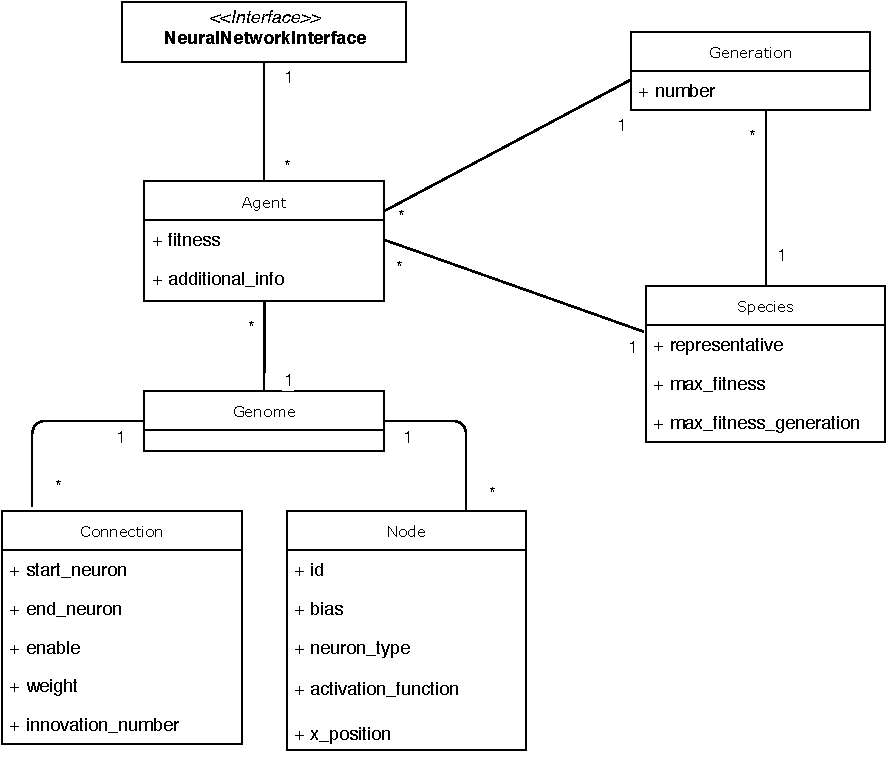
\includegraphics[width=1\textwidth]{./img/uml/class_diagramm.pdf} 
	\caption{UML-Diagramm mit den verwendeten Datenstrukturen}
	\label{fig:class_diagramm}
\end{figure}
\\ \noindent
Die erste Klasse ist das \emph{Genome}, welches das aus Kapitel \ref{sec:neat} bekannte Genom repräsentiert und alle Informationen zur Konstruktion eines \ac{KNN} besitzt. Hierfür werden zwei Listen benötigt, wobei die erste alle Neuronen und die zweite alle Verbindungen des \ac{KNN} enthält. Diese Repräsentation entspricht der Kodierung aus Kapitel \ref{subsec:neat_encoding}. 
\\\\
Ein Neuron wird durch die Klasse \emph{Node} repräsentiert und enthält unter anderem den \emph{Bias}-Wert sowie die zu verwendende Aktivierungsfunktion, welche für die Berechnungen im \ac{KNN} benötigt werden. Zusätzlich sind zur Vereinfachung der späteren Implementierung der beschriebenen Anforderungen einige weitere Werte wie der Neuronentyp vorhanden. Dies vereinfacht die spätere Visualisierung sowie das Einsetzen der Eingabewerte und das Auslesen des Ausgabevektors. Zusätzlich besitzt jedes Neuron eine x-Koordinate, welche die relative x-Position für eine spätere Visualisierung angibt. Die \emph{Input}- und \emph{Output}-Neuronen besitzen die Werte $0$ und $1$. Die \emph{Hidden}-Neuronen werden, wie in Kapitel \ref{subsec:neat_minimal_structure} beschrieben, nur durch strukturelle Mutationen hinzugefügt und dabei zwischen zwei anderen Neuronen platziert. Die x-Koordinate von diesen wird berechnet, indem der Mittelwert der zwei anderen Neuronen gebildet wird. Zuletzt enthält jedes Neuron zur Identifizierung eine ID, welche von den Verbindungen genutzt wird.
\\\\
Eine Verbindung zwischen zwei Neuronen wird im Genom durch eine Instanz der Klasse \emph{Connection} repräsentiert. Sie enthält jeweils die ID des Startneurons sowie des Zielneurons. Zusätzlich ist das Gewicht sowie ein Aktivierungsbit gegeben. Letzteres gibt entsprechend der vorgestellten Kodierung an, ob die Verbindung im \ac{KNN} enthalten sein soll. Die letzte Variable ist die Innovationsnummer, welche in Kapitel \ref{subsec:neat_reproduction} beschrieben, durch strukturelle Mutationen zugewiesen und in der Reproduktionsphase zum Lösen des \emph{Competing Conventions} Problems verwendet wird.
\\\\
In Kapitel \ref{sec:evolutionary_algos} ist der Begriff des Individuums erläutert. In dieser Arbeit werden diese durch Instanzen der Klasse \emph{Agent} repräsentiert und sind nach dem Agenten benannt, welcher beim bestärkenden Lernen mit der Umwelt interagiert. Der hierbei erhaltene Fitnesswert, welcher im späteren Verlauf die Selektion maßgeblich beeinflusst, wird in der entsprechenden Variable \emph{fitness} gespeichert. Das Datenfeld \emph{additional\_info} kann Zusatzinformationen enthalten, welche vom Optimierungsproblem stammen können.
\\\\
Die zwei letzten Klassen in diesem Diagramm sind die \emph{Generation} und \emph{Species}. Bei Letzterem handelt es sich, wie aus Kapitel \ref{subsec:neat_species} bekannt, um eine Gruppierung ähnlicher Individuen bzw. Agenten. Entsprechend der in Kapitel \ref{subsec:neat_species} enthaltenen Definition ist eine Spezies durch ein Genom repräsentiert und besitzt eine Mitgliederliste. Zusätzlich wird der höchste erreichte Fitnesswert des besten Mitglieds gespeichert sowie die Generation, in welcher dieser Wert erzielt wurde. Dies wird benötigt, um den Fortschritt zu überwachen, da eine Spezies, deren Mitglieder keine Steigerung des Fitnesswertes in einer festgelegten Anzahl an Generationen erzielen, nicht für die Reproduktion ausgewählt wird.
\\\\
Die aus Kapitel \ref{subsec:evolutionary_algorithm} bekannte Generation ist durch die Klasse \emph{Generation} repräsentiert und enthält je eine Liste für alle Individuen sowie für alle verschiedenen Spezies. Zusätzlich wird sie durch eine Nummer identifiziert, welche angibt, wie viele Zyklen der Evaluation, Selektion, Rekombination und Mutation bereits durchgeführt worden sind.

\subsubsection{Künstliches neuronales Netz}
Aus dem Genom wird ein \ac{KNN}, dessen Aufbau und Funktionsweise in Kapitel \ref{sec:neuroal_networks} ausführlich erläutert sind, erstellt, welches dann im Optimierungsproblem eingesetzt wird. Prinzipiell können hierfür verschiedene bereits implementierte Bibliotheken verwendet werden wie beispielsweise \emph{Tensorflow} \cite{tensorflow2015} oder \emph{PyTorch} \cite{pytorch2019}. Mit diesen können vor allem rein ebenenweise verbundene \ac{KNN}, wie in Kapitel \ref{subsec:network_structures} vorgestellt, schnell und einfach erstellt werden. Allerdings können durch \ac{NEAT} auch \ac{KNN} mit \emph{shortcut} Verbindungen entstehen sowie Netze mit Rückkopplungen. Zwar kann die Funktionalität von diesen auch mit \emph{Tensorflow} und \emph{PyTorch} abgebildet werden, aber dafür ist ein entsprechend höherer Implementierungsaufwand notwendig, der im Rahmen dieser Arbeit nicht umgesetzt wird. Stattdessen wird eine eigene vereinfachte Implementierung verwendet. Ein Nachteil von dieser besteht darin, dass sie im Vergleich zu Implementierungen aus großen Bibliotheken insgesamt langsamer ist. Der Grund hierfür ist, dass die Bibliotheken gut optimiert sind und auch die Verwendung von \acp{GPU} unterstützen, welche die benötigte Ausführungszeit stark reduzieren können. Auch wenn im Folgenden statt großer Bibliotheken die eigene Implementierung verwendet wird, soll ein Grundgerüst erstellt werden, sodass eine spätere Integration einfach möglich ist. Dies wird mit einem Interface realisiert, welches die grundlegenden Funktionen definiert. Sowohl die in dieser Arbeit verwendete Implementierung als auch zukünftige Erweiterungen können dieses nutzen und ermöglichen somit ein einfaches Austauschen der verschiedenen Implementierungen. Das Interface definiert drei Funktionen mit den Namen \emph{build()}, \emph{reset()} und \emph{activate()}. Die \emph{build()} Funktion konstruiert aus einem an sie übergebenen Genom ein \ac{KNN}, die \emph{activate()} Funktion produziert aus einer ihr übergebenen Liste mit Eingabewerten den Ausgabevektor. Die Anzahl an Eingabe- und Ausgabewerten entspricht dabei der Anzahl an \emph{Input}- und \emph{Output}-Neuronen im \ac{KNN}. Bei der \emph{reset()} Funktion werden zuletzt eventuell gespeicherte Ergebnisse, wie sie bei einem Netz mit Rückkopplungen enthalten sein können, entfernt und auf den Startwert zurückgesetzt. 
\\\\
Die in dieser Arbeit verwendete \emph{BasicNeuralNetwork} Implementierung setzt dieses Interface mit dem Ziel um, \ac{KNN} sowohl mit als auch ohne Rückkopplungen berechnen zu können. Da eine genaue Beschreibung der Implementierung nicht von Interesse ist, wird an dieser Stelle nur der oberflächliche Ablauf beschrieben. Bei der \emph{build()} Funktion wird je eine Liste für die \emph{Input}- und \emph{Output}-Neuronen angelegt, in welche die Neuronen mit den entsprechenden Typen sortiert werden. Eine dritte Liste enthält alle im \ac{KNN} enthaltenen Neuronen. Jedes Neuron speichert zudem eine Liste mit den Verbindungen, welche zu ihm führen und den aktuellen sowie letzten berechneten Wert. Die letzte Aufgabe dieser Funktion ist die Festlegung der Reihenfolge, in welcher die einzelnen Neuronen aktiviert bzw. deren Zwischenergebnisse berechnet werden. Bei der Reihenfolge ist zu beachten, dass bei einem Netz ohne Rückkopplung jedes vorherige Neuron bis zu den \emph{Input}-Neuronen bereits aktiviert sein muss, da ansonsten das Ergebnis verfälscht wird. Bei Netzen mit Rückkopplungen gilt diese Anforderung, außer für Verbindungen, welche in derselben Schicht oder von Neuronen der nachfolgenden Schichten ausgehen, prinzipiell auch. Dies sind Rückkopplungen, bei welchen der zuletzt berechnete Wert zurückgegeben wird, sodass keine Endlosschleife entsteht. 
\\\\
Bei der \emph{activate()} Funktion wird ein Eingabevektor an das \ac{KNN} übergeben. Jeder darin enthaltene Wert wird in ein \emph{Input}-Neuron gesetzt. Dies ist mit der zuvor in der \emph{build()} Funktion erstellten Liste aller \emph{Input}-Neuronen effizient umzusetzen. Danach beginnt die eigentliche Berechnung des Ausgabevektors. Hierzu werden die Neuronen in der zuvor festgelegten Reihenfolge aktiviert bzw. berechnet. Zuletzt wird der Ausgabevektor erstellt. Auch dies ist effizient umsetzbar, da zuvor eine Liste mit allen \emph{Output}-Neuronen erstellt wurde. Über diese wird iteriert und die entsprechenden Ergebnisse in eine neue Liste kopiert, welche schlussendlich den Ausgabevektor repräsentiert und als Ergebnis der Funktion zurückgegeben wird. Die \emph{reset()} Funktion iteriert über die Liste mit allen Neuronen und entfernt die gespeicherten Zwischenergebnisse. 

\subsubsection{Optimierungsproblem}
In den vorherigen Kapiteln sind die grundlegenden Datenstrukturen und die Funktionalität des \ac{KNN} vorgestellt. Bevor das eigentliche Optimierungsverfahren implementiert werden kann, wird noch das Optimierungsproblem als grundlegende Komponente benötigt. Wie in Kapitel \ref{subsub:optimzation_problem} vorgestellt, können diese Optimierungsprobleme aus verschiedenen Domänen stammen und sich sehr voneinander unterscheiden. Somit muss auch für dieses ein Interface erstellt werden, das möglichst viele Szenarien abbilden kann, welche einfach und mit wenig Aufwand durch das in dieser Arbeit implementierte Verfahren optimierbar sind.
\\\\
Das Interface enthält fünf Funktionen, von denen lediglich die \emph{evaluate()} Funktion immer benötigt wird. Die restlichen vier Funktionen sind optional und können je nach Optimierungsproblem zusätzlich eingesetzt werden. Im Folgenden wird auf die Bedeutung aller Funktionen genauer eingegangen. Die \emph{initialization()} Funktion kann zum Initialisieren der Umgebung verwendet werden und wird einmalig zu Beginn durch die später vorgestellte Bibliothek aufgerufen. Dies kann beispielsweise verwendet werden, um notwendige Daten initial aus einer Datenbank zu laden oder um die Umgebung zu erstellen. Ist die Initialisierung abgeschlossen, können prinzipiell verschiedene Agenten in dieser evaluiert werden. Vor jeder Evaluation wird die \emph{before\_evaluation()} Funktion aufgerufen, mit welcher beispielsweise der Zustand der Umgebung zurückgesetzt werden kann, sodass jeder Agent denselben Startzustand vorfindet. Danach wird die eigentliche Evaluation mit der Funktion \emph{evaluate()} durchgeführt, die als die wichtigste Funktion in diesem Interface zu beschreiben ist und notwendigerweise für jedes Optimierungsproblem implementiert werden muss. Als Parameter wird ein initialisiertes \ac{KNN} übergeben, welches mit dem Genom eines Agenten erstellt wurde. Mit diesem soll das Optimierungsproblem gelöst werden. Die genaue Implementierung dieser Funktion kann je nach Problem sehr unterschiedlich sein. Verschiedene Beispiele werden in Kapitel \ref{chap:analysis} genauer vorgestellt. Bei der Implementierung ist zu beachten, dass die Funktion zwei Rückgabewerte erwartet. Der erste ist vom Typ \emph{float} und repräsentiert den erreichten Fitnesswert. Wie in Kapitel \ref{subsub:optimzation_problem} vorgestellt, bewertet dieser die Leistung des \ac{KNN} und wird für die spätere Selektionsphase benötigt. Der zweite Rückgabewert ist vom Typ \emph{Dict} und kann verschiedene \emph{Key-Value} Paare mit Zusatzinformationen des Optimierungsproblems enthalten. Diese werden letztendlich im Datenfeld \emph{additional\_info} des Agenten gespeichert, welches in Kapitel \ref{subsubsec:data_structures} vorgestellt ist. Die darin gespeicherten Daten können für eine spätere Auswertung sowie in der Abbruchbedingung für den Algorithmus verwendet werden. Nach jeder durchgeführten Evaluation wird das Pendant zur \emph{before\_evaluation()} Funktion ausführt, die \emph{after\_evaluation()} Funktion.  Mit dieser sowie der letzten in diesem Interface enthaltenen Funktion \emph{clean\_up()} können verschiedene Tätigkeiten zur Freigabe von Ressourcen oder Wiederherstellung des originalen Zustands der Umgebung umgesetzt werden. Der Unterschied zwischen diesen Funktionen ist, dass die \emph{clean\_up()} Funktion das Pendant zur \emph{initialization()} Funktion ist und nur einmalig am Ende des Trainingsverfahren aufgerufen wird. 
 
\subsubsection{Schnittstelle der Bibliothek}
\label{subsubsec:library_interface}
Nachdem die für diese Arbeit benötigten Komponenten vorgestellt sind, kann auf die Schnittstelle der Bibliothek genauer eingegangen werden. Ziel ist, dass diese die grundlegenden Funktionen definiert, welche sowohl von der sequenziellen als auch der parallelisierten Implementierung umgesetzt werden. Somit bieten beide Implementierungen dieselben Funktionalitäten, können einfach ausgetauscht werden und ermöglichen einen einfachen Vergleich. 
\begin{figure}[!h]
	\centering
	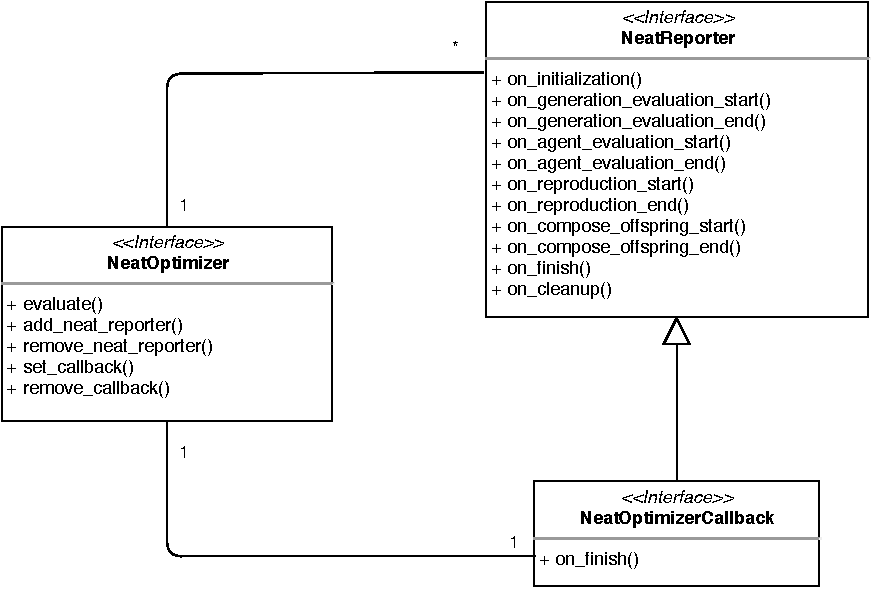
\includegraphics[width=0.8\textwidth]{./img/uml/uml-library_interface.pdf} 
	\caption{Interfaces für die Schnittstelle der Bibliothek}
	\label{fig:library_interface}
\end{figure}
\\ \noindent
Die Schnittstelle der Bibliothek besteht aus drei Interfaces, die als \emph{NeatOptimizer}, \emph{NeatReporter} und \emph{NeatOptimizerCallback} bezeichnet werden und deren Beziehung zueinander in Abbildung \ref{fig:library_interface} dargestellt ist. Zu erkennen ist, dass der \emph{NeatOptimizerCallback} vom \emph{NeatReporter} erbt und somit dessen Funktionalität erweitert. Der \emph{NeatOptimizer} besitzt genau einen \emph{NeatOptimizerCallback} sowie beliebig viele \emph{NeatReporter}. Auf die Funktionalität von diesen wird später genauer eingegangen. Im Folgenden wird zuerst der \emph{NeatOptimizer} betrachtet, welcher fünf Funktionen besitzt, von denen vier für das Hinzufügen und Entfernen von Instanzen der Klassen \emph{NeatReporter} und \emph{NeatOptimizerCallback} verwendet werden. Die letzte Funktion hat den Namen \emph{evaluate()}, startet den Ablauf des Optimierungsproblems und erhält als Parameter die hierfür benötigten Werte. Die ersten beiden Parameter bestimmen die Anzahl der \emph{Input}- und \emph{Output}-Neuronen und somit die Größe des Eingabe- und Ausgabevektors. Da der Optimierungsvorgang in \ac{NEAT}, wie in Kapitel \ref{subsec:neat_minimal_structure}  beschrieben, mit einer minimalen Struktur beginnt, sind keine \emph{Hidden}-Neuronen anzugeben. Der nächste Parameter ist eine Referenz auf eine Aktivierungsfunktion, welche von allen Neuronen verwendet wird. Einige bekannte Vertreter, von denen ein Teil in Kapitel \ref{subsubsec:activatoin_function} vorgestellt ist, sind standardmäßig in diesem Projekt enthalten, wobei das Hinzufügen von weiteren Funktionen jederzeit möglich ist. Hierauf folgt der Parameter \emph{challenge}, der eine Klasse repräsentiert, die das Interface des Optimierungsproblems implementiert. Der Algorithmus versucht, das hierin enthaltene Problem zu optimieren. Die zuletzt zu betrachtenden Parameter sind mit \emph{config} und \emph{seed} bezeichnet. Letzterer soll die Generierung der Zufallswerte beeinflussen und somit den Optimierungsvorgang wiederholbar und vergleichbar machen. Die \emph{config} repräsentiert eine Konfiguration, in welcher verschiedene Parameter des Verfahrens spezifiziert sind. In dieser wird beispielsweise angegeben, wie hoch die Chance auf eine strukturelle Mutation ist oder wie sehr sich die Gewichte der Verbindungen ändern können. Auf die tatsächlich verwendeten Konfigurationen wird im Rahmen der Analyse in Kapitel \ref{chap:analysis} weiter eingegangen.
\\\\
Das Ausführen der \emph{evaluate()} Funktion startet den gesamten Optimierungsprozess, welcher je nach Komplexität eine Laufzeit von mehreren Stunden oder Tagen haben kann. Häufig ist es in diesen Anwendungsfällen gewünscht, Zwischenergebnisse und Fortschritte anzuzeigen, sodass die verbleibende Laufzeit und der Erfolg des Verfahrens besser abschätzbar sind. Dies wird in dieser Arbeit durch Callbacks realisiert, welche durch die Interfaces \emph{NeatReporter} und \emph{NeatOptimizerCallback} implementiert werden. Das Interface \emph{NeatReporter} definiert einige Funktionen, welche während der Laufzeit des Algorithmus regelmäßig an bestimmten Punkten aufgerufen werden. Klassen, die diese implementieren, können hierdurch Statusinformationen über den aktuellen Zustand sowie den Fortschritt des Verfahrens erhalten. Das Interface wird in dieser Arbeit unter anderem für die regelmäßige Speicherung des besten Agenten und zur Messung der Performance genutzt. Die erste hierbei implementierte Funktion ist \emph{on\_initialization()}, welche einmalig zu Beginn aufgerufen wird. Das Pendant hierzu ist die \emph{on\_cleanup()} Funktion, welche einmalig am Ende aufgerufen wird. Auch für die Zwischenzeit gibt es einige Funktionen, die den Beginn und das Ende verschiedener Phasen signalisieren. Die Funktionen \emph{on\_generation\_evaluation\_start()} und \emph{on\_generation\_evaluation\_end()} werden zum Beginn und Ende der Evaluationsphase aufgerufen. Als Parameter wird an beide Funktionen die aktuell evaluierte Generation übergeben, sodass sie zum Nachverfolgen des besten und durchschnittlichen Fitnesswertes verwendet werden kann. Mit den Funktionen \emph{on\_agent\_evaluation\_start()} und \emph{on\_agent\_evaluation\_end()} wird angegeben, wann die Evaluierung eines einzelnen Agenten beginnt und abgeschlossen ist. An diese Funktion wird der eigentliche Agent sowie ein Index übergeben, welcher angibt, wie viele Evaluationen in dieser Generation bereits durchgeführt wurden. Diese Informationen können beispielsweise für einen Fortschrittsbalken verwendet werden. Die Funktionen \emph{on\_reproduction\_start()} und \emph{on\_reproduction\_end()} markieren den Beginn und das Ende der Reproduktionsphase, welche mit der Selektion startet und mit dem Ersetzen der vorherigen Generation durch die neu erstellten Agenten endet. Um die Zeit zu messen, welche für die Rekombination und Mutation eines einzelnen neuen Agenten benötigt wird, sind die Funktionen \emph{on\_compose\_offsprings\_start()} und  \emph{on\_compose\_offsprings\_end()} enthalten. Die letzte in diesem Interface enthaltene Funktion ist mit \emph{on\_finish()} bezeichnet und erhält als Parameter die aktuelle Generation. Sie wird einmalig am Ende der Optimierung aufgerufen, nachdem die Abbruchbedingung erfüllt ist. Diese kann verwendet werden, um das beste \ac{KNN} und die erhaltenen Ergebnisse zu visualisieren und zu speichern.
\\\\
Die Klasse \emph{NeatOptimizerCallback} erbt vom Interface \emph{NeatReporter} und kann daher alle bereits vorgestellten Funktionen nutzen. Diese sind für den Programmablauf optional und werden nicht zwingend benötigt. Dies trifft nicht auf die Funktion \emph{finish\_evaluation()} zu, welche im \emph{NeatOptimizerCallback} als einzige zusätzlich implementiert ist. Sie bekommt die aktuelle Generation als Parameter übergeben und gibt einen Wert vom Typ \emph{boolean} zurück, womit die Abbruchbedingung umgesetzt wird. Die Funktion wird nach Beendigung der Evaluationsphase mit der aktuellen Generation sowie mit allen erzielten Fitnesswerten aufgerufen. Ist das Ergebnis der Funktion \emph{True}, wird die Ausführung des Algorithmus beendet und die entsprechenden Callback Funktionen \emph{on\_finish()} und \emph{on\_cleanup()} aufgerufen. Liefert die Funktion \emph{False}, wird mit der Selektion, Rekombination und Mutation fortgefahren und der Zyklus startet erneut. Diese Art der Abbruchbedingung ermöglicht vielfältige Umsetzungen. Zum Beispiel kann der Algorithmus beendet werden, wenn der Fitnesswert eines Agenten einen Schwellwert übersteigt, eine gewisse Anzahl an Zyklen bzw. Generationen durchgeführt oder eine festgelegte Trainingszeit überschritten ist.

\subsubsection{Serviceklassen}
Ein wichtiges Ziel bei der Entwicklung ist das Einsparen von unnötigem Implementierungsaufwand, so auch in dieser Arbeit. Aus diesem Grund wurden die bereits vorgestellten Interfaces erstellt, welche sowohl von der sequenziellen als auch der parallelisierten Implementierung verwendet werden. Der Vorteil hierdurch ist, dass ein einfaches Austauschen und Vergleichen der beiden Verfahren möglich ist. Die eigentliche Implementierung unterscheidet sich zwangsläufig in einigen Aspekten. Dennoch wird ein großer Teil der Komponenten von \ac{NEAT} gleich bleiben, da sich die Funktionen nicht durch eine Parallelisierung ändern. Aus diesem Grund wird ein Großteil dieser Funktionen als Serviceklassen implementiert, die keinen internen Zustand besitzen und somit zwei Vorteile bieten. Erstens ist es einfach möglich, die Funktionen in verschiedenen Implementierungen zu nutzen. Zweitens ermöglicht eine solche Struktur ein einfaches automatisiertes Testen der Implementierung. Dies ist besonders wichtig, da Fehler im Trainingsverfahren zu einem späteren Zeitpunkt aufgrund der Größe der Population schwer zu lokalisieren sind.
\\\\
Insgesamt werden drei Serviceklassen mit den Bezeichnungen \emph{GenerationService}, \emph{ReproductionService} und \emph{SpeciesService} erstellt, welche Funktionen entsprechend ihrer Benennung übernehmen. So befasst sich die erste Klasse mit allen Funktionen, welche die ganze Generation betreffen, die zweite mit Funktionen bezüglich des Erstellens und Modifizierens von Genomen sowie Agenten und die letzte Klasse mit Funktionen bezüglich der verschiedenen Spezies. Im Folgenden wird auf die jeder Serviceklasse zugeordneten Funktionen genauer eingegangen. Allerdings sei hierzu angemerkt, dass keine genauen Implementierungsdetails vorgestellt werden. Die theoretische Funktionalität ist in den Kapiteln \ref{sec:evolutionary_algos} und  \ref{sec:neat} erläutert. Für die genaue praktische Umsetzung wird auf den veröffentlichten Programmcode verwiesen.
\\\\
Der \emph{ReproductionService} besitzt vor allem Funktionen, um neue Genome mittels Reproduktion zu erzeugen oder bestehende zu mutieren. Die erste Funktion, \emph{cross\_over()}, setzt die eigentliche Reproduktion insofern um, dass in ihr zwei Elterngenome verwendet werden, um einen Nachkommen zu erzeugen. Grundsätzlich entsprechen sowohl die Umsetzungen dieser Funktion als auch die der anderen in diesem Kapitel vorgestellten Funktionen den Erläuterungen der vorherigen Kapitel. Eine Besonderheit soll an dieser Stelle hervorgehoben werden. Ein wichtiges Ziel für ein wiederholbares Ergebnis ist, dass unabhängig von einem Prozess mit demselben \emph{Seed} immer dasselbe Ergebnis erzielt wird. Dies ist mit einem einfachen globalen Zufallsgenerator in einem verteilten System nicht möglich, weshalb für jedes Genom ein neuer Zufallsgenerator erzeugt wird, dessen \emph{Seed} sich aus den beiden Elterngenomen ergibt und welcher für alle Zufallsoperationen verwendet wird, die dieses Genom betreffen. Der hieraus resultierende Vorteil ist, dass unabhängig vom Prozess und dessen internem Zustand dieselben Eltern immer denselben Nachkommen produzieren. Der hierfür erstellte Zufallsgenerator wird zudem für die Funktionen \emph{mutate\_weights()}, \emph{mutate\_add\_connection()} und \emph{mutate\_add\_node()} verwendet. Die erste Funktion mutiert die Gewichte aller Verbindungen, die zweite fügt dem Genom eine neue Verbindung und die dritte ein neues Neuron hinzu. Bei Letzterem werden entsprechend der Definition in Kapitel \ref{subsec:neat_mutation} zusätzlich zwei neue Verbindungen erstellt.
\\\\
Die Klasse \emph{GenerationService} besitzt einige Funktionen zum Erzeugen der initialen Population. Wie in der Schnittstellendefinition beschrieben, wird anfänglich nur die Anzahl an \emph{Input}- und \emph{Output}-Neuronen übergeben. Die Funktion \emph{create\_genome\_structure()} erzeugt mit diesen Informationen eine Struktur für das \ac{KNN}, welche die entsprechenden Neuronen und Verbindungen enthält. Mithilfe der Funktion \emph{create\_initial\_generation()} kann mit der generierten Struktur eine neue Generation erstellt werden. Hierfür wird das Genom für jeden zu erstellenden Agenten einmal kopiert und die Gewichte der Verbindungen zufällig gesetzt. Schlussendlich werden die Agenten in einem letzten Schritt den Spezies zugeordnet.
\\\\
Der \emph{SpeciesService} besitzt im Vergleich zum \emph{GenerationService} bedeutend mehr Funktionen. Um die erstellten Agenten den verschiedenen Spezies zuzuordnen, kann die Funktion \emph{sort\_agents\_into\_species()} genutzt werden. Entsprechend der Erläuterung in Kapitel \ref{subsec:neat_species} iteriert diese über die Liste mit allen Agenten und überprüft für jeden die Kompatibilität mit den existierenden Spezies. Der Kompatibilitätswert zwischen zwei Genomen kann mithilfe der Funktion \emph{calculate\_genetic\_distance()} berechnet werden. Ist dieser kleiner als ein konfigurierter Schwellwert, wird der Agent der Spezies zugeordnet. Existiert keine passende Spezies, wird eine neue erstellt. Dies sind aber nicht die einzigen Funktionen. In Kapitel \ref{subsec:neat_species} ist das \emph{explicit fitness sharing} Verfahren eingeführt worden, welches mit der Funktion \emph{calculate\_adjusted\_fitness()} umgesetzt ist. Der angepasste Fitnesswert wird schließlich bei der Selektion verwendet, welche mit den Funktionen \emph{calculate\_amount\_offspring()} und \emph{create\_offspring\_pairs()} umgesetzt ist. Die erste Funktion berechnet, wie viele Nachkommen jede Spezies erhalten soll. Die zweite Funktion erstellt die tatsächlichen Elternpaare, welche zum Erzeugen der Nachkommen verwendet werden. Zuletzt sind noch einige kleinere Funktionen enthalten. Bei \ac{NEAT} können nur die besten $50\%$ der Genome zur Reproduktion ausgewählt werden, die Funktion \emph{remove\_low\_genomes()} entfernt die restlichen. Nach jeder Generation wird zudem ein neues Genom zur Repräsentation jeder Spezies ausgewählt. Dies ist in diesem Projekt mit der Funktion \emph{select\_new\_representative()} umgesetzt. Die letzten beiden Funktionen heißen \emph{reset\_species()} und \emph{get\_species\_with\_members()}. Die erste hiervon entfernt alle Mitglieder einer Spezies. Dies wird typischerweise durchgeführt, bevor die neu erstellten Agenten den Spezies zugewiesen werden. Nach der Zuweisung wird die zweite Funktion aufgerufen. Diese filtert Spezies heraus, welche keine Mitglieder zugewiesen bekommen haben und entfernt diese aus der Liste. 

\subsubsection{Performance Messung}
Es gibt verschiedene Kriterien, um die Performance eines neuroevolutionären Algorithmus zu beurteilen. In der Literatur, so auch in Quelle \cite{stanley2002evolving}, wird häufig die Anzahl an Generationen in Kombination mit der Populationsgröße angegeben, bis eine Lösung für ein Optimierungsproblem gefunden ist. Hiermit kann die Anzahl der evaluierten \ac{KNN} abgeleitet werden und ein Vergleich zu anderen Verfahren ist möglich. In vielen Fällen ist dies sinnvoller als ein direkter Vergleich der tatsächlichen Laufzeiten, da diese sehr von der verwendeten Hardware, Programmiersprache und der effizienten Implementierung abhängig sind bzw. beeinflusst werden können. Auch in dieser Arbeit wird diese Art der Performance Messung mit der Klasse \emph{FitnessReporter} durchgeführt, die von der bereits vorgestellten Klasse \emph{NeatReporter} erbt und damit unter anderem Zugriff auf die Funktion \emph{on\_generation\_evaluation\_end()} hat. Der \emph{FitnessReporter} legt für jede Generation einen Datensatz an, in welchem sowohl der durchschnittliche als auch beste Fitnesswert gespeichert wird. Hierdurch ist einerseits ersichtlich, wie viele Generationen der Algorithmus benötigt, und zusätzlich kann der Fortschritt zwischen den einzelnen Generationen betrachtet werden. Dies kann wertvolle Erkenntnisse liefern, wenn der Algorithmus schlechter oder langsamer ist als erwartet. 
\\\\
In dieser Arbeit spielt auch die tatsächlich benötigte Ausführungszeit eines Algorithmus, welche auch als \emph{wall clock time} bezeichnet wird, eine große Rolle. Im Rahmen dieser Arbeit werden die Zeiten erfasst und dienen als Basis für den Vergleich zwischen der sequenziellen und parallelisierten Implementierung. Hierfür wird die Klasse \emph{TimeReporter} erstellt, welche ebenfalls das Interface \emph{NeatReporter} implementiert und Zugriff auf die verschiedenen bereits vorgestellten Funktionen hat. Mit diesen können die benötigten Ausführungszeiten für verschiedene Phasen des Algorithmus erfasst werden. Auf die genaue Unterteilung wird im Rahmen von Kapitel \ref{chap:analysis} genauer eingegangen. 

\subsubsection{Visualisierung}
Die verschiedenen erfassten Messwerte sollen für eine bessere und einfachere Auswertung graphisch dargestellt werden können. Der beste Fitnesswert pro Generation soll in einem Liniendiagramm und die erfassten Ausführungszeiten in einem Säulendiagramm dargestellt werden. Bei Letzterem sollen die verschiedenen Phasen aufeinandergestapelt visualisiert sein. Dies hat den Vorteil, dass sowohl das Verhältnis der verschiedenen Phasen zueinander als auch die gesamte Ausführungszeit über mehrere Generationen hinweg ausgewertet werden kann. Für diese Diagramme soll das Paket \emph{Matplotlib} für die Sprache Python verwendet werden \cite{pyplot2007hunter}. Dieses ermöglicht ein einfaches und schnelles Erstellen von diversen Diagrammtypen und ist zusätzlich sehr gut in die Entwicklungsumgebung PyCharm integriert, welche im Rahmen dieser Arbeit verwendet wird.
\\\\
Zusätzlich zu den Diagrammen sollen auch die erstellten \ac{KNN} visualisiert werden, was eine größere Herausforderung darstellt. Eine mögliche Umsetzung, welche in diesem Rahmen evaluiert wird, nutzt die Software \emph{Graphviz} \cite{graphviz2000gansner}. Diese besitzt eine eigene Beschreibungssprache, welche als \emph{DOT} bezeichnet wird und die Beschreibung von verschiedene Graphentypen ermöglicht. Würde ein \ac{KNN} in dieser Arbeit mit \emph{Graphviz} visualisiert werden, müssten die im  Genom kodierten Informationen im \emph{DOT} Format in eine Textdatei exportiert werden und erst danach mithilfe von \emph{Graphviz} als PDF oder Bildatei erstellt werden. Da dieser Vorgang verhältnismäßig aufwendig ist, wird eine alternative Lösung mithilfe des Pythonpakets NetworkX umgesetzt \cite{networkx2008hagberg}. Dieses wird normalerweise primär für die Analyse von Graphen eingesetzt, ermöglicht allerdings auch die Visualisierung dieser. Als Basis hierfür verwendet das Paket entweder die vorgestellte Software \emph{Graphviz} oder alternativ \emph{Matplotlib}. 
Letzteres bietet sich   an, da es bereits in diesem Projekt verwendet wird und eine bessere Integration in die Entwicklungsumgebung bietet. Allerdings müssen auch bei diesem Verfahren die im Genom enthaltenen Informationen in einem gewissen Format an das Paket übergeben werden. Eine weitere Herausforderung bei der Implementierung ist, dass die Knoten des Graphen, in diesem Fall die Neuronen, normalerweise eine zufällige Position zugewiesen bekommen und daher keine Darstellung der Schichten möglich ist. Um diese zu erhalten, müssen sämtliche Positionen manuell berechnet werden. Hierbei ist das Bestimmen der x-Koordinate einfach, da diese für jedes Neuron bereits im Genom gespeichert ist. Die y-Koordinate wird dann in Abhängigkeit von der Anzahl an weiteren Neuronen in derselben Schicht bestimmt.    

\subsubsection{Persistenz}
Die persistente Speicherung der Optimierungsergebnisse ist die letzte zu nennende Anforderung an die Implementierung dieser Arbeit. Dies umfasst sowohl die Speicherung der Genome als auch die der Performance Ergebnisse. Für die Speicherung der Daten wurden prinzipiell zwei Ansätze evaluiert. Beim ersten Ansatz würde eine klassische SQL- oder NoSQL-Datenbank zur Speicherung eingesetzt werden. Der Vorteil von einem solchen System ist, dass viele Nutzer gleichzeitig auf die Daten zugreifen können. Dies ist allerdings für den gegebenen Anwendungskontext nicht notwendig und der Aufwand, welcher durch die Implementierung der verschiedenen Anfragen entsteht, im Vergleich zur zweiten Variante bedeutend höher.
\\\\
Der zweite Ansatz ist bedeutend einfacher. Das Ziel ist, dass die Ergebnisse nur in einer lokalen Datei gespeichert bzw. aus einer solchen Datei geladen werden können. Ein solches Vorgehen bietet einige Vorteile. Der erste ist, dass ein geringer Implementierungsaufwand notwendig ist. Das standardmäßig in Python enthaltene \emph{Pickle} Modul erfüllt genau diese Voraussetzungen. Es bietet sowohl vorgefertigte Funktionen zum Serialisieren von unterschiedlichen Objekten in Python an, welche dann in einer Datei gespeichert werden können, als auch Funktionen zum Laden solcher Datensätze. Zwei Vorteile von diesem Verfahren sind, dass der programmiertechnische Aufwand sehr gering ist und dass trainierte Modelle als Datei vorliegen, wodurch sie auf \emph{GitHub} oder ähnlichen Plattformen einfach veröffentlicht werden können.
\\\\
Das eigentliche Speichern soll auf jeden Fall am Ende das Trainingsverfahrens durchgeführt werden. Allerdings kann es zusätzlich sinnvoll sein, in regelmäßigen Abständen die bis dahin erhaltenen Zwischenergebnisse ebenfalls zu sichern. Hierfür gibt es verschiedene Gründe. Bei einer ungünstigen Konfiguration kann ein Trainingsverfahren eventuell niemals die Abbruchbedingung erfüllen. In diesem Fall müsste das Programm manuell abgebrochen werden, wobei sämtliche Ergebnisse verloren gingen. Auch Implementierungsfehler können zu einem Absturz führen, bei welchem nicht die finalen Ergebnisse gespeichert werden. Bei der parallelisierten Implementierung können zusätzlich Hardware- und Netzwerkfehler auftreten, für die \ac{MPI}, wie in Kapitel \ref{subsubsec:hpc_architecture} beschrieben, anfällig ist. Aus diesem Grund wird die Klasse \emph{CheckPointReporter} implementiert, welche ebenfalls das Interface \emph{NeatReporter} umsetzt. Hierbei werden die Funktionen \emph{on\_generation\_evaluation\_end()} und \emph{on\_finish()} implementiert, wobei bei Aufruf von letzterer das finale Ergebnis immer gespeichert wird. Bei der \emph{on\_generation\_evaluation\_end()} Funktion ist es abhängig von der gewählten Konfiguration. In dieser wird spezifiziert, nach wie vielen Generationen ein Zwischenergebnis abgespeichert werden soll. Prinzipiell ist es möglich, sowohl nach jeder Generation die Ergebnisse zu speichern als auch gar nicht, wobei Letzteres nicht zu empfehlen ist.

\section{Sequenzielle Implementierung}
\label{sec:sequential_implementation}
Im vorherigen Kapitel sind die verschiedenen Komponenten dieser Arbeit vorgestellt, welche zur Implementierung des sequenziellen Verfahrens verwendet werden. Der grundsätzliche Ablauf entspricht hierbei den Erläuterungen der Kapitel \ref{sec:evolutionary_algos} und \ref{sec:neat}. Daher wird in diesem Kapitel hauptsächlich auf die technische Umsetzung sowie das Zusammenspiel der bereits vorgestellten Komponenten eingegangen. 
\\\\
Die \emph{evaluate()} Funktion ist, wie in Kapitel \ref{subsubsec:library_interface} beschrieben, der Einstiegspunkt für die Bibliothek. Initial werden die bereits spezifizierten \emph{NeatReporter} und der \emph{NeatOptimizerCallback} mit der Funktion \emph{on\_initialization()} über den Beginn des Verfahrens informiert. Direkt im Anschluss wird auch das Optimierungsproblem initialisiert und die erste Generation erstellt. Danach beginnt der Zyklus aus Evaluation, Selektion, Rekombination und Mutation. Hierfür wird zuerst die \emph{evaluate\_generation()} Funktion aufgerufen, deren Implementierung im weiteren Verlauf noch genauer erläutert wird. Grundsätzlich werden die verschiedenen Agenten im Optimierungsproblem evaluiert und erhalten einen Fitnesswert. Nach Abschluss dieser Phase wird überprüft, ob das Verfahren beendet werden soll, indem die Funktion \emph{finish\_evaluation()} des \emph{NeatOptimizerCallbacks} aufgerufen wird. Ist dies der Fall, wird die Schleife abgebrochen, die finale Generation zurückgegeben und die \emph{NeatReporter} sowie der \emph{NeatOptimizerCallback} darüber informiert. Andernfalls wird mit der Funktion \emph{build\_new\_generation()} eine neue Population durch die Phasen Selektion, Rekombination und Mutation erstellt, worauf in diesem Kapitel ebenfalls noch genauer eingegangen wird. 
\\\\
Am Anfang der \emph{evaluate\_generation()} Funktion werden die \emph{NeatReporter} und der \emph{NeatOptimizerCallback} über den Beginn der Evaluationsphase informiert. Im Anschluss wird über alle Agenten iteriert und für jeden die Evaluation durchgeführt. Dies umfasst das Aufrufen der entsprechenden Funktionen im \emph{NeatOptimizerCallback} und den \emph{NeatReportern} sowie das Erstellen und Evaluieren des \ac{KNN}.
\\\\
In der \emph{build\_new\_generation()} Funktion ist der Großteil der Funktionalität von \ac{NEAT} enthalten, dementsprechend aufwendig ist die Implementierung. Zu Beginn werden wie bei der  \emph{evaluate\_generation()} Funktion die \emph{NeatReporter} und der \emph{NeatOptimizerCallback} über den Beginn dieser Phase informiert. Danach werden entsprechend der originalen Publikation von \ac{NEAT} die besten Genome jeder Spezies mit mehr als $x$ Mitglieder selektiert und unverändert in die nächste Generation kopiert, wobei $x$ ein konfigurierbarer Schwellwert ist. Im Anschluss wird über jede Spezies iteriert und der höchste erreichte Fitnesswert aktualisiert, sofern sich dieser in der letzten Generation geändert hat. Dies ist für den nächsten Schritt wichtig, da bei diesem die Spezies entfernt werden, welche keine Fitnesssteigerung in den letzten $t$ Generationen erzielt haben, wobei auch $t$ konfigurierbar ist. Die Mitglieder der entsprechenden Spezies können in der nachfolgenden Selektion nicht als Elternteile ausgewählt werden.
\\\\
Für die verbleibenden Spezies wird im Anschluss der angepasste Fitnesswert berechnet und auf Basis von diesem im darauffolgenden Schritt die Anzahl an Nachkommen bestimmt. Bevor es zur eigentlichen Selektion kommt, werden zusätzlich noch die Agenten entfernt, welche im vorherigen Durchlauf schlechte Fitnesswerte erzielt haben. Diese können somit nicht für die Reproduktion ausgewählt werden. Nachdem diese Schritte durchgeführt sind, kann die eigentliche Selektion mit der Funktion \emph{create\_offspring\_pairs()} beginnen. Im Rahmen dieser Funktion wird über jede Spezies iteriert und für jeden zu erzeugenden Nachkommen zwei Elternteile zufällig ausgewählt, welche als Paar in einer Liste zwischengespeichert werden. Anhand dieser Liste wird die Rekombination und Mutation durchgeführt. Durch die Funktion \emph{cross\_over()} wird die Rekombination implementiert, welche das Genom für den Nachkommen erzeugt. Anschließend wird das Genom mithilfe der nacheinander aufgerufenen Funktionen \emph{mutate\_weights()}, \emph{mutate\_add\_node()} und \emph{mutate\_add\_connection()} mutiert.
\\\\
Vor der Zuordnung der neu erstellten Agenten in die Spezies müssen noch zwei weitere Funktionen ausgeführt werden. Zuerst wird für jede Spezies die \emph{select\_new\_representative()} Funktion aufgerufen, welche ein Mitglied zufällig auswählt und dessen Genom als Repräsentanten setzt. Danach werden durch den Aufruf der Funktion \emph{reset\_species()} alle bisherigen Mitglieder entfernt. Erst an dieser Stelle werden die neuen Agenten auf Basis ihres Kompatibilitätswertes tatsächlich den verschiedenen Spezies zugeordnet. Zuletzt werden in der \emph{build\_new\_generation()} Funktion die Spezies entfernt, welche keine Mitglieder erhalten haben. Danach wird die neue Generation erstellt und als Ergebnis der Funktion zurückgegeben. 

